\documentclass[12pt]{article}
\usepackage{amscd,amssymb,amsthm,amsxtra,exscale,latexsym,verbatim,paralist}
\usepackage{mathrsfs}
\usepackage[T1]{fontenc}
\usepackage{newtxmath,newtxtext}
\usepackage[left = 2cm, top = 2cm, bottom = 2cm, right = 2cm]{geometry}

\usepackage{hyperref}
\usepackage{tikz}
\usetikzlibrary{patterns}

\newcommand{\XB}{\color{black}}
\newcommand{\XBB}{\color{blue}}
\newcommand{\XV}{\color{violet}}
\newcommand{\XR}{\color{red}}
\newcommand{\ds}{\displaystyle}

\setlength{\parindent}{0pt} 
\setlength{\parskip}{\baselineskip}

\theoremstyle{plain}
\newtheorem{ex}{Exercise}

\renewcommand{\proofname}{Solution}

\begin{document}

\title{\textbf{MTH385}: History of Mathematics - Homework \#4}
\date{\today}
\author{\XV\textit{\large{\href{https://github.com/casonk}{Cason Konzer}}}\XB}

\maketitle

\hrulefill

\newpage

\begin{center}
  The simplest epicyclic curve is the \emph{cardioid} (``heart-shape''), which results from a circle rolling on a fixed circle of the same size.
\end{center}

\begin{center}
  \begin{tikzpicture}[scale=3]
    \draw (0,0) circle (1);
    \draw [blue, loosely dotted] (2,0) circle (1);
    \draw [blue, dotted]  (1.414,1.414) circle (1);
    \draw [blue, loosely dashed]  (0,2) circle (1);
    \draw [blue, dashed]  (-2,0) circle (1);
    \draw [blue]  (0,-2) circle (1);
    \draw[->, loosely dashed] (0.9,1.9) to[out=90, in=0] (0,2.9);
    \draw[->, dashed] (-2,0.9) to[out=180, in=90] (-2.9,0);
    \draw[->] (0,-2.9) to[out=0, in=-90] (0.9,-2);
    \draw [ultra thick, violet, domain=-3.141:3.141, samples=250, variable=\t] plot ({1*(2*cos(\t r) - cos(2*\t r))},{1*(2*sin(\t r) - sin(2*\t r))});
    \draw [fill, blue] (1.414,0.414) circle [radius=0.025];
    \draw [fill, blue] (1,2) circle [radius=0.025];
    \draw [fill, blue] (1,-2) circle [radius=0.025];
    \draw [fill, blue] (1,0) circle [radius=0.025];
    \draw [fill, blue] (-3,0) circle [radius=0.025];
  \end{tikzpicture}

  Cardioid
\end{center}

\begin{center}
  \begin{tikzpicture}[scale=3.5]
    \draw (0,0) circle (1);
    \draw [blue] (2,0) circle (1);
    \draw (0,0) -- (1,0);
    \draw [blue] (2,0) -- (1,0);
    \draw [fill] (1,0) circle [radius=0.035];
    \draw [fill, blue] (1,0) circle [radius=0.025];
  \end{tikzpicture}

  Cardioid construction $ \theta = 0 $
\end{center}

\begin{center}
  \begin{tikzpicture}[scale=3.5]
    \draw (0,0) circle (1);
    \draw [blue]  (1.414,1.414) circle (1);
    \draw (0,0) -- (0.707,0.707);
    \draw [dashed] (0,0) -- (1,0);
    \draw [dotted] (0,0) -- (0,1);
    \draw [blue, dashed] (1.414,1.414) -- (0.707,0.707);
    \draw [blue, dotted] (1.414,1.414) -- (0.414,1.414);
    \draw [blue] (1.414,1.414) -- (1.414,0.414);
    \draw [fill, blue] (1.414,0.414) circle [radius=0.025];
    \node [below, blue] at (1.414,0.414) {$t$};
    \draw [] (1,0) circle [radius=0.035];
    \draw [blue] (1,0) circle [radius=0.025];
    \draw [fill] (0.707,0.707) circle [radius=0.035];
    \node [right, blue] at (1,0) {$t_{0}$};
    \node [above right] at (0.1,0) {$\theta$};
    \node [below left] at (0,0) {$O$};
    \node [below left, blue] at (1.314,1.414) {$\theta$};
    \node [below left, blue] at (1.414,1.314) {$\theta$};
    \node [above right, blue] at (1.414,1.414) {$C$};
  \end{tikzpicture}

  Cardioid construction $ \theta = \pi/4 $
\end{center}

\newpage
%%%%%%%%%%%%%%%%%%%%%%%%%%%%%%%%%%%%%%%%%%%%%%%%%%%%%%%%%%%%%%%%%%%%%%%%%%%%%%%%%%%%%%%%%%%%%%%%%%%%%%%%%%%%%
%%%%%%%%%%%%%%%%%%     #1     %%%%%%%%%%%%%%%%%%%%%%%%%%%%%%%%%%%%%%%%%%%%%%%%%%%%%%%%%%%%%%%%%%%%%%%%%%%%%%%
%%%%%%%%%%%%%%%%%%%%%%%%%%%%%%%%%%%%%%%%%%%%%%%%%%%%%%%%%%%%%%%%%%%%%%%%%%%%%%%%%%%%%%%%%%%%%%%%%%%%%%%%%%%%%

\XBB\hrulefill\XB \\
\begin{ex} [2.5.4]
  Show that if both circles have radius $ 1 $, and we follow the point on the rolling circle initially at $ (1, 0) $, then the cardioid it traces out has parametric equations
  \begin{align*}
    x &= 2\cos\theta-\cos2\theta, \\
    y &= 2\sin\theta-\sin2\theta.
  \end{align*}
\end{ex}
\XBB\hrulefill\XB \\

\begin{proof}
  \ \\

  From the above two examples we can see that the distance between the origin of the two circles will always be $ 2 $ as it is the sum of their radii.

  \begin{itemize}
    \item The point $ C $ will thus always be at $ 2 (\cos(\theta), \sin(\theta)) $.
    \item The ``tracer'' of the cardioid is the blue dot and will always be at $ C - (\cos(\pi + 2\theta), \sin(\pi + 2\theta)) $.
    \item We now have an equation for $ t $ : $ t = (2\cos(\theta) - \cos(\pi + 2\theta), 2\sin(\theta) - \sin(\pi + 2\theta)) $.
    \item Decomposing we have $ x = 2\cos(\theta) - \cos(\pi + 2\theta) $ and $ y = 2\sin(\theta) - \sin(\pi + 2\theta) $.
  \end{itemize}
    We will now simply using sum and difference identities to arrive at the parametric equations. 
    \begin{itemize}
    \item $ \cos(\pi + 2\theta) = \cos(\pi)\cos(2\theta) - \sin(\pi)\sin(2\theta) = \cos(2\theta) $.
    \item $ \sin(\pi + 2\theta) = \sin(\pi)\cos(2\theta) - \cos(\pi)\sin(2\theta) = \sin(2\theta) $.
    \item $ x = 2\cos\theta - \cos2\theta $.
    \item $ y = 2\sin\theta - \sin2\theta $.
  \end{itemize}

  \begin{center}
    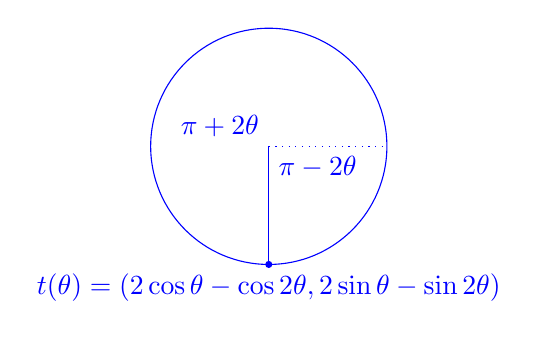
\begin{tikzpicture}[scale=1.5]
      \draw [blue]  (1.414,1.414) circle (1);
      \draw [blue] (1.414,1.414) -- (1.414,0.414);
      \draw [blue, dotted] (1.414,1.414) -- (2.414,1.414);
      \draw [fill, blue] (1.414,0.414) circle [radius=0.025];
      \node [below, blue] at (1.414,0.414) {$t(\theta) = (2\cos\theta - \cos2\theta, 2\sin\theta - \sin2\theta)$};
      \node [above left, blue] at (1.414,1.414) {$\pi + 2\theta$};
      \node [below right, blue] at (1.414,1.414) {$\pi - 2\theta$};
    \end{tikzpicture}
  
    $ t(\pi/4) $
  \end{center}

\end{proof}

\newpage

\begin{center}
  The cardioid is an algebraic curve. Its cartesian equation may be hard to discover, but it is easy to verify, especially if one has a computer algebra system.
\end{center}

%%%%%%%%%%%%%%%%%%%%%%%%%%%%%%%%%%%%%%%%%%%%%%%%%%%%%%%%%%%%%%%%%%%%%%%%%%%%%%%%%%%%%%%%%%%%%%%%%%%%%%%%%%%%%
%%%%%%%%%%%%%%%%%%     #2     %%%%%%%%%%%%%%%%%%%%%%%%%%%%%%%%%%%%%%%%%%%%%%%%%%%%%%%%%%%%%%%%%%%%%%%%%%%%%%%
%%%%%%%%%%%%%%%%%%%%%%%%%%%%%%%%%%%%%%%%%%%%%%%%%%%%%%%%%%%%%%%%%%%%%%%%%%%%%%%%%%%%%%%%%%%%%%%%%%%%%%%%%%%%%
\XBB\hrulefill\XB \\
\begin{ex} [2.5.5]
  Check that the point $(x,y)$ on the cardioid satisfies
  \[
    (x^2+y^2-1)^2=4((x-1)^2+y^2).
  \]
\end{ex}
\XBB\hrulefill\XB \\

\begin{proof}
  \ \\

  We will use substitution for this exercise

  \begin{itemize}
    \item $ (x^{2} + y^{2} - 1)^{2} = 4((x-1)^{2} + y^{2}) $.
    \item $ x^{2} = (2\cos\theta - \cos2\theta)^{2} = 4\cos^{2}\theta - 4\cos\theta\cos2\theta + \cos^{2}2\theta $.
    \item $ y^{2} = (2\sin\theta - \sin2\theta)^{2} = 4\sin^{2}\theta - 4\sin\theta\sin2\theta + \sin^{2}2\theta $.
    \item $ x^{2} + y^{2} - 1 = 4\cos^{2}\theta + 4\sin^{2}\theta - 4\cos\theta\cos2\theta - 4\sin\theta\sin2\theta + \cos^{2}2\theta + \sin^{2}2\theta - 1 $.
    \subitem $ = 4 - 4(\cos(\theta - 2\theta)) = 4 - 4\cos\theta $.
    \item $ (x^{2} + y^{2} - 1)^{2} = 16\cos^{2}\theta - 32\cos\theta + 16 $.
    \item $ (x-1)^{2} = (2\cos\theta - \cos2\theta -1)^2 $.
    \subitem $ = 4\cos^{2}\theta + \cos^{2}2\theta - 4\cos\theta\cos2\theta - 4\cos\theta + 2\cos2\theta + 1 $.
    \item $ (x-1)^{2} + y^{2} = $ 
    \subitem $ 4\cos^{2}\theta + 4\sin^{2}\theta + \cos^{2}2\theta + \sin^{2}2\theta + 1 - 4\cos\theta\cos2\theta - 4\sin\theta\sin2\theta - 4\cos\theta + 2\cos2\theta $.
    \subitem $ = 6 - 4\cos\theta - 4\cos\theta + 2\cos2\theta $.
    \subitem $ = 6 - 8\cos\theta + 2(2\cos^{2}\theta - 1) $.
    \subitem $ = 4\cos^2\theta - 8\cos\theta + 4 $.
    \item $ 4((x-1)^{2} + y^{2}) = 16\cos^{2}\theta - 32\cos\theta + 16 $ .
  \end{itemize}

  We can now see that any point satisfying our parametric equations also satisfies the algebragic equality.

\end{proof}

\newpage
%%%%%%%%%%%%%%%%%%%%%%%%%%%%%%%%%%%%%%%%%%%%%%%%%%%%%%%%%%%%%%%%%%%%%%%%%%%%%%%%%%%%%%%%%%%%%%%%%%%%%%%%%%%%%
%%%%%%%%%%%%%%%%%%     #3     %%%%%%%%%%%%%%%%%%%%%%%%%%%%%%%%%%%%%%%%%%%%%%%%%%%%%%%%%%%%%%%%%%%%%%%%%%%%%%%
%%%%%%%%%%%%%%%%%%%%%%%%%%%%%%%%%%%%%%%%%%%%%%%%%%%%%%%%%%%%%%%%%%%%%%%%%%%%%%%%%%%%%%%%%%%%%%%%%%%%%%%%%%%%%
\XBB\hrulefill\XB \\
\begin{ex} [3.2.3]
  Show that the $k^{th}$ pentagonal number is $ \ds \frac{3k^{2} - k}{2} $.
\end{ex}
\XBB\hrulefill\XB \\

\begin{proof}
  \ \\

  We have the $k^{th}$ pentagonal number represented as the sum : $ \ds pent_{k} = \sum_{i = 1}^{k} 3i - 2 $. \\

  From the summation we notice that $ pent_{k + 1} = pent_{k} + 3(k + 1) - 2 = pent_{k} + 3k + 1 $. \\

  Similarly, $ pent_{k + 2} = pent_{k + 1} + 3(k + 2) - 2 = pent_{k} + 3k + 1 + 3(k + 2) - 2 = pent_{k} + 6k + 5 $.

  Thus if the equality holds we have show that $ \ds \frac{3k^{2} - k}{2} $ is a closed form for $ pent_{k} $.

  \begin{itemize}
    \item For base $ pent_{0} + 3(0) + 1 = pent_{1} $.
    \subitem $ \ds \frac{3(0)^{2} - 0}{2} + 3(0) + 1 = 0 + 0 + 1 = 1 $.
    \item For base $ pent_{0} + 6(0) + 5 = pent_{2} $.
    \subitem $ \ds \frac{3(0)^{2} - 0}{2} + 6(0) + 5 = 0 + 0 + 5 = 5 $.
    \item To show $ pent_{k} + 3k + 1 = pent_{k + 1} $.
    \subitem $ \ds \frac{3k^{2} - k}{2} + 3k + 1 = \frac{3k^{2} + 6k -k + 2}{2} = \frac{(3k^{2} +6k -3) + (- k - 1)}{2} = \frac{3(k + 1)^{2} - (k + 1)}{2} $.
    \item To show $ pent_{k} + 6k + 5 = pent_{k + 2} $.
    \subitem $ \ds \frac{3k^{2} - k}{2} + 6k + 5 = \frac{3k^{2} + 12k -k + 10}{2} = \frac{(3k^{2} +12k -12) + (- k - 2)}{2} = \frac{3(k + 2)^{2} - (k + 2)}{2} $.
  \end{itemize}

  Thus induction shows that the $k^{th}$ pentagonal number is $ \ds \frac{3k^{2} - k}{2} $.

\end{proof}

\newpage
%%%%%%%%%%%%%%%%%%%%%%%%%%%%%%%%%%%%%%%%%%%%%%%%%%%%%%%%%%%%%%%%%%%%%%%%%%%%%%%%%%%%%%%%%%%%%%%%%%%%%%%%%%%%%
%%%%%%%%%%%%%%%%%%     #4     %%%%%%%%%%%%%%%%%%%%%%%%%%%%%%%%%%%%%%%%%%%%%%%%%%%%%%%%%%%%%%%%%%%%%%%%%%%%%%%
%%%%%%%%%%%%%%%%%%%%%%%%%%%%%%%%%%%%%%%%%%%%%%%%%%%%%%%%%%%%%%%%%%%%%%%%%%%%%%%%%%%%%%%%%%%%%%%%%%%%%%%%%%%%%
\XBB\hrulefill\XB \\
\begin{ex} [3.2.4]
  Show that each square is the sum of two consecutive triangular numbers.
\end{ex}
\XBB\hrulefill\XB \\

\begin{proof}
  \ \\

  We have the $k^{th}$ triangular number represented as the sum : $ \ds tri_{k} = \sum_{i = 1}^{k} i $. \\

  The $k^{th}$ triangular number has the well know closed form : $ \ds tri_{k} = \frac{k(k + 1)}{2} $. \\

  We have the $l^{th}$ square number represented as the sum : $ \ds sq_{l} = \sum_{j = 1}^{l} 2l -1 $. \\

  The $l^{th}$ square number has the well know closed form : $ \ds sq_{l} = l^{2} $. \\

  \begin{itemize}
    \item We now consider two consecutive triangular numbers, $ tri_{k} $ and $ tri_{k + 1} $.
    \subitem $ \ds tri_{k} + tri_{k + 1} = \frac{k(k + 1)}{2} + \frac{(k + 1)(k + 2)}{2} = \frac{k^{2} + k + k^{2} + 2k + k + 2}{2} $.
    \subitem $ \ds = \frac{2k^{2} + 4k + 2}{2} = k^{2} + 2k + 1 = (k + 1)^{2} $.
    \item considering $ l = k + 1 $
    \subitem $ l^{2} = tri_{l-1} + tri_{l} \ ; \ \forall l \ge 1 $.
  \end{itemize}

  We have shown that each square, $ sq_{l} $, is the sum of the coresponding consecutive triangular numbers, $ tri_{l-1} $, and $ tri_{l} $.

\end{proof}

\newpage

\begin{center}
  Euclid's theorem about perfect numbers depends on the prime divisor property, which will be proved in the next section. Assuming this for the moment, it follows that if $ 2^{n} - 1 $ is a prime $ p $, then the proper divisors of $ 2^{n - 1}p $ (those unequal to $ 2^{n - 1}p $ itself) are \dots
\end{center}
\[
  1,2,2^2,\ldots,2^{n - 1}\text{ and }p,2p,2^{2}p,\ldots,2^{n - 2}p.
\]

%%%%%%%%%%%%%%%%%%%%%%%%%%%%%%%%%%%%%%%%%%%%%%%%%%%%%%%%%%%%%%%%%%%%%%%%%%%%%%%%%%%%%%%%%%%%%%%%%%%%%%%%%%%%%
%%%%%%%%%%%%%%%%%%     #5     %%%%%%%%%%%%%%%%%%%%%%%%%%%%%%%%%%%%%%%%%%%%%%%%%%%%%%%%%%%%%%%%%%%%%%%%%%%%%%%
%%%%%%%%%%%%%%%%%%%%%%%%%%%%%%%%%%%%%%%%%%%%%%%%%%%%%%%%%%%%%%%%%%%%%%%%%%%%%%%%%%%%%%%%%%%%%%%%%%%%%%%%%%%%%
\XBB\hrulefill\XB \\
\begin{ex} [3.2.5]
  Given that the divisors of $ 2^{n - 1}p $ are those just listed, show that $ 2^{n - 1}p $ is perfect when $ p = 2^{n} - 1 $ is prime.
\end{ex}
\XBB\hrulefill\XB \\

\begin{proof}
  \ \\

  We must show that the sum of the proper divisors of $ 2^{n - 1}p $ is equal to $ 2^{n - 1}p $, let $ \Sigma $ denote this sum.\\

  We will let $ q = 2^{n - 1}p $ \dots

  \begin{itemize}
    \item $ \ds \Sigma = \Sigma_{1} + \Sigma_{2} = (2^{0} + 2^{1} + \dots + 2^{n-1}) + p(2^{0} + 2^{1} + \dots + 2^{n-2}) $.
    \item $ \ds \Sigma + q = \Sigma_{1} + \Sigma_{2} + q = (2^{0} + 2^{1} + \dots + 2^{n-1}) + p(2^{0} + 2^{1} + \dots + 2^{n-1}) = \Sigma_{1} + p\Sigma_{1} $.
    \item $ \ds \Sigma_{1} + p\Sigma_{1} = \Sigma_{1}(1 + p) = \Sigma_{1}(1 + 2^{n} - 1) = 2^{n}\Sigma_{1} $.
    \item As $ \Sigma_{1} $ is a geometric progression, $ \Sigma_{1} = 2^{n} - 1 = p $.
    \item Thus $ \Sigma + q = 2^{n}p = 2(2^{n-1}p) = 2q $.
    \item Finally $ \Sigma = q $.
  \end{itemize}

  We have now shown that $ q = 2^{n - 1}p $ is perfect.

\end{proof}




\end{document}

